\begin{frame} \frametitle{Grappa Tree}
	A structure designed to store a forest supporting the following operations: \\
	Make-Tree, Link, Cut, Evert, Left-Mark, Right-Mark, Oracle-Search. \\
	Each of them is performed in $O(\log n)$. \\ \bigskip
	Uses heavy-path decomposition. \\ \bigskip
	Voronoi Diagram is stored as a Grappa tree with face-markers \\
	on each edge: cells of which sites are to the right / left from it.
\end{frame}

\begin{frame} \frametitle{Procedure}
\begin{enumerate}
	\item Evert the tree so that the root is at infinity, \medskip
	\item Identify portion of each heavy path inside $\text{\scshape cell} (q, S_{\text{new}})$, \medskip
	\item Within each path find non-preserved edges, \medskip
	\item Remove all non-preserved edges, \medskip
	\item Link back the resulting components in the right order.
\end{enumerate}
\end{frame}

\begin{frame} \frametitle{Dynamic Circle Reporting Structure} \label{pg:dcr}
	We need to report all the circles from the set containing a given point. \\
	Lift the circles to planes
	$$(x,y)\ \mapsto\ (x,y,x^2+y^2).$$ \vspace{-0.4cm}
	
	Using point-plane duality in $\mathbb R^3$ the circle-reporting can be reduced to \\
	extreme-point query that Chan's structure is originally designed for. \bigskip
	
	The DCR has far-going applications. We store roots of heavy paths $\Psi$ \\
	in this structure.
\end{frame}

\begin{frame} \frametitle{Finding Non-Preserved Edges}
	For each root $r \in \Psi_q$ (returned by the DCR) {\it transition edge} $h_r$ is computed in $O(\log n)$. \\ [0.8cm]
\begin{center}
	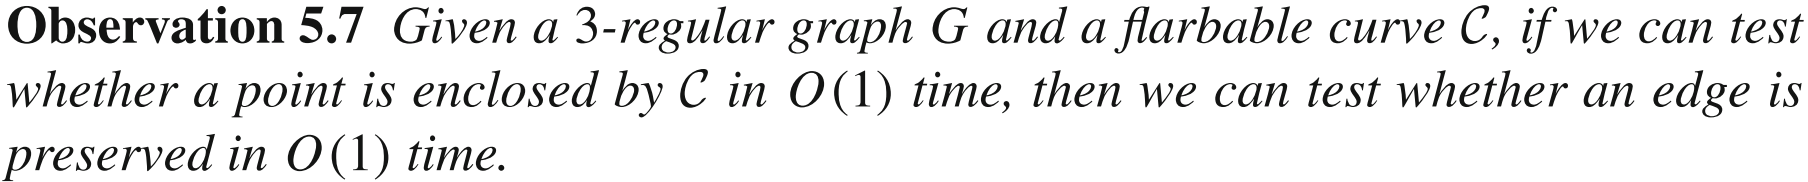
\includegraphics[width=14cm]{figs/5-7.png} \\ [0.7cm]
\end{center}
	We can now proceed to finding {\it all} non-preserved edges.
\end{frame}

\begin{frame} \frametitle{Shadow edges. Bent edges.} \vspace{-2mm}
	$\mathcal V_q (S)$ — all the edges of the diagram that intersect the face $\text{\scshape cell} (q, S_\text{new})$ \\
	of new site. \medskip
	
	{\it Shadow edge} is an edge among these that is not preserved. We can mark \\
	all shadow edges in $O(|\Psi_q| \log n)$. There are also {\it bent edges} that can't \\
	be preserved. They need to be marked. 

\begin{center}
	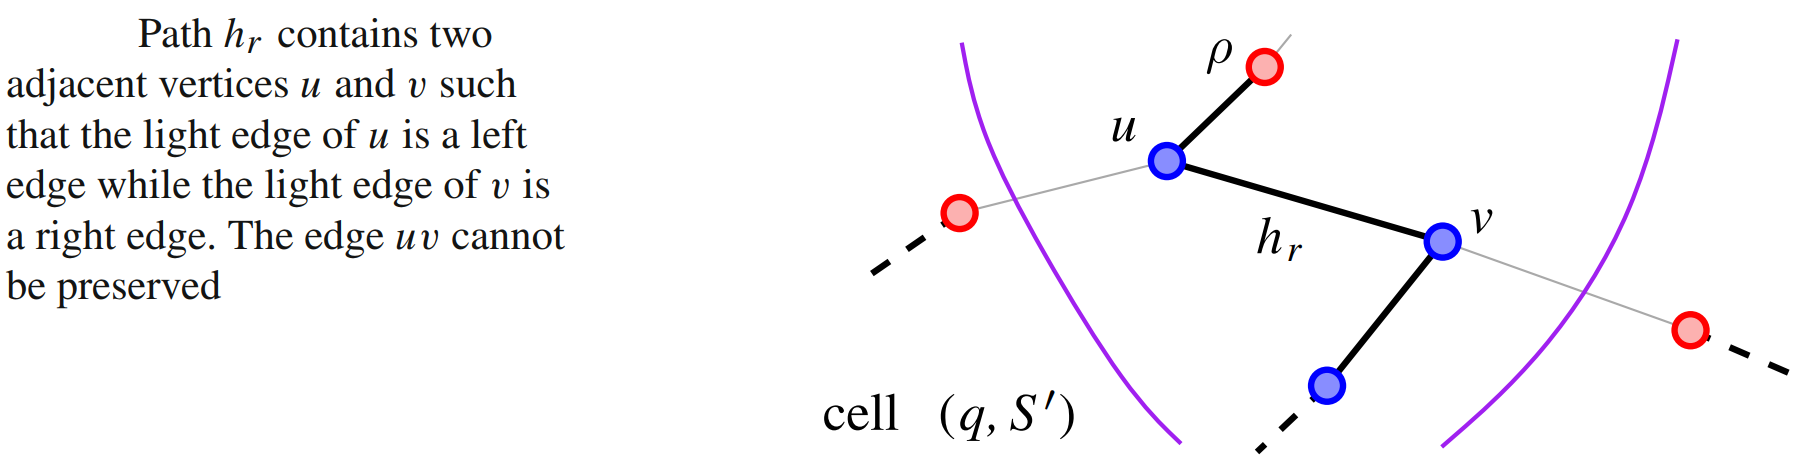
\includegraphics[width=11.5cm]{figs/bent.png} \vspace{-3mm}
\end{center}

	After all, the edge is preserved iff it is not marked as shadow.
\end{frame}

\begin{frame} \frametitle{Compressed Tree} \label{pg:compres}
	$\mathcal F$ — forest obtained after {\it (virtually)} removing all shadow edges. Each component of it is a {\it comb.} Combs can be large, but we want to have a tour on the graph to see how to re-link it. So we compress each comb into a supernode. \medskip

	If $\sigma$ is a number of shadow edges, the compressed tree has $O(\sigma)$ vertices / edges and can be obtained in $O(\sigma \log \sigma)$. \smallskip

\begin{center}
	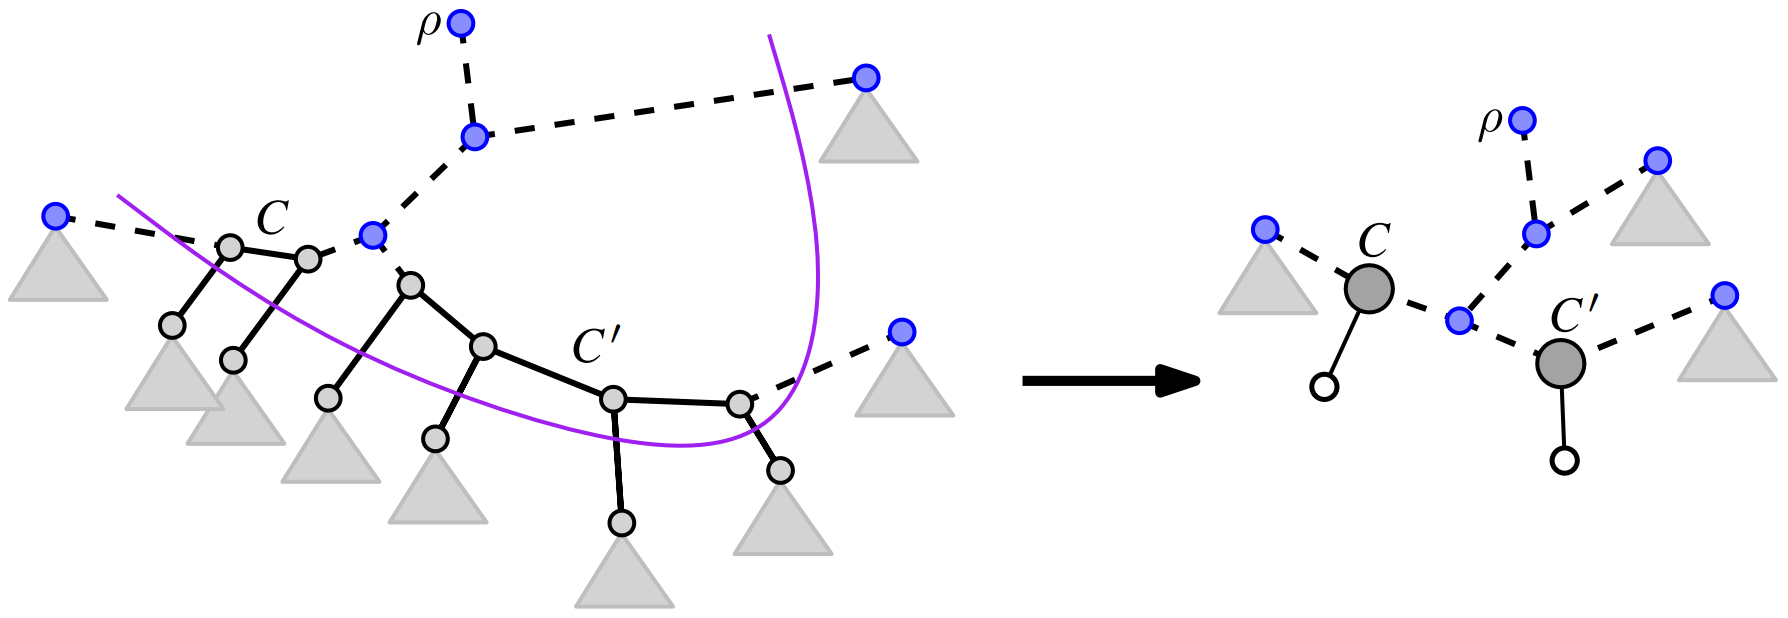
\includegraphics[width=9.8cm]{figs/compres}
\end{center}
\end{frame}

\begin{frame} \frametitle{Decompression}
\begin{center}
	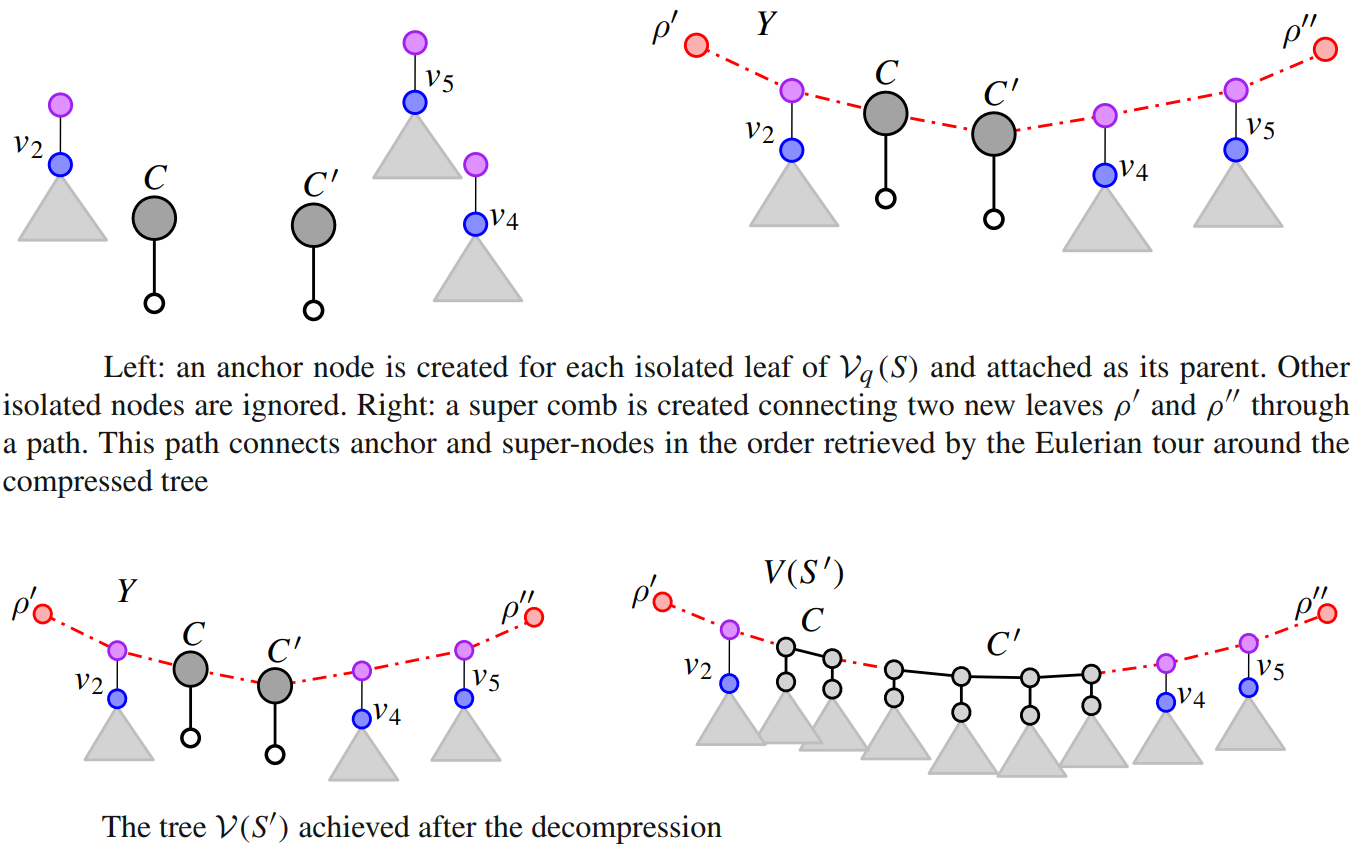
\includegraphics[width=11cm]{figs/decompres}
\end{center}
\end{frame}